% \chapter{Classificação de Intensidade das Emoções na Fala em Português Brasileiro por meio de Deep Learning}\label{Cap:Pesquisa}

% Este capítulo irá se desdobrar a partir do problema encontrado e proporá uma solução para sua realização. Independente de formação enquanto profissionais de saúde mental, é natural que consigamos atribuir alguma espécie de métrica para comparar duas instâncias de uma mesma emoção que tenhamos sentido. Assim, conseguimos experienciar e comparar intensidades distintas para uma mesma emoção. Portanto, somos capazes de identificar emoções, quantificar sua intensidade e calcular uma distância para poder efetuar essa comparação. Conforme visto, trabalhos de \textit{ML} aplicados ao reconhecimento de emoções na fala vêm sendo publicados - ao menos - desde o início da década de 90 (1990), e se tornam menos frequentes quando buscamos por tarefas mais especializadas.\\

% Este capítulo irá se desdobrar a partir do problema encontrado e proporá uma solução para sua realização. Adiante, irá expor a sua implementação em detalhes, tratando conhecimentos mais específicos que não estejam elucidados ao longo dos capítulos anteriores e conjecturando sobre possíveis aplicabilidades deste trabalho em áreas diversas.\\

Este capítulo apresenta uma arquitetura para classificação da intensidade da emoção na voz em Português. Para tal, foram criados dois modelos de \acrshort{DL}, a saber: (i) \acrshort{AE}, responsável pela redução de dimensionalidade e extração de características representativas dos dados; e (ii) Rede Neural, para efetuar a predição da classe relativa a intensidade da vocalização.\\


% ==========================================================================================
\section{Visão Geral}

Na Figura \ref{fig:visaogeralproposta} é apresentada uma visão geral da arquitetura. Conforme a imagem, três etapas principais serão necessárias para o reconhecimento da intensidade das emoções: (A) Aquisição de informações; (B) Extração de características; e (C) Classificação da intensidade.

\begin{figure}[]
\centering
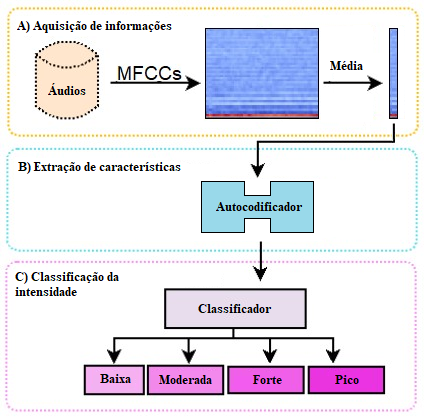
\includegraphics[width=0.60\textwidth]{img/arquitetura-visao-geral-3.png}
\caption{\label{fig:visaogeralproposta}Visão geral da arquitetura}
\end{figure}

A primeira etapa (A) lida com a obtenção dos dados que serão utilizados no dissertação e da sua conversão para uma interpretação passível de utilização por modelos de aprendizagem de máquina. Podemos descrever os dados como um conjunto de registros rotulados que serão utilizados para treinamento e teste dos modelos implementados na proposta.

A segunda etapa (B) lida com a extração de características dos dados convertidos. Essas características serão obtidas através de um modelo não supervisionado para a redução de dimensionalidade e posteriormente utilizadas como entrada de um modelo supervisionado de classificação da intensidade da emoção.

A terceira e última etapa (C) é responsável pela inferência da intensidade. O modelo recebe as características obtidas na etapa anterior e realiza o treinamento e testagem do modelo de classificação de acordo com quatro classes possíveis: (i) Baixa; (ii) Moderada; (iii) Forte; e (iv) Pico de intensidade.

Este projeto aplicará esta arquitetura em dois cenários modelados a serem detalhados no capítulo posterior, juntamente com os resultados obtidos.

% ==========================================================================================
% \section{Aquisição dos dados}

% O primeiro passo para tarefas de \acrlong{ML} que envolvem \acrshort{SER} costuma ser a aquisição dos dados que serão utilizados pelo modelo. Em virtude do escopo da proposta, necessitamos de um \textit{dataset} em português que possua as classes desejadas: Emoção e intensidade. Até o momento da escrita deste trabalho, não conhecemos algum \textit{dataset} que seja ideal (idioma, emoções e intensidade) para esta proposta. Então, este trabalho utilizará duas bases de dados: VERBO~\cite{12.21} e VIVAE~\cite{16}.

% O primeiro \textit{dataset}, VERBO, é composto por vocalizações verbais, acomodando todos os fonemas da língua portuguesa, com exemplos para seis emoções básicas (alegria, nojo, medo, raiva, surpresa, tristeza) e um estado emocional denominado de neutro. O segundo, VIVAE, é composto por vocalizações não verbais distribuídas em seis classes (conquista, prazer sexual, surpresa positiva, raiva, medo e dor física), com exemplos em quatro intensidades (baixa, moderada, forte e pico de intensidade). Graças a fusão de domínios~\cite{49}, conseguimos o cenário da Tabela \ref{table:datasetideal}.

% ==========================================================================================
\section{Aquisição de informações da base de conhecimento}\label{section:basesdedados}

Para modelar a intensidade da emoção, uma das dificuldades é a falta de dados rotulados~\cite{18}. Tradicionalmente, em áreas como visão computacional ou reconhecimento de voz, os \textit{datasets} chegam a ter milhões de registros, como, por exemplo: ImageNet (imagem) com  mais de 14 milhões e Google AudioSet (áudio) com mais de 2 milhões de amostras. Podemos ver um comparativo na Tabela \ref{table:comparativodbs} entre datasets populares~\cite{32} em trabalhos de \acrshort{SER}: AudioSet, Berlin Database of Emotional Speech (EMO-DB)~\cite{32.55}, Danish emotional speech database (DES)~\cite{32.56}, The Ryerson Audio-Visual Database of Emotional Speech and Song (RAVDESS)~\cite{32.57}, Toronto Emotional Speech Set (TESS)~\cite{32.58} e Crowd-Sourced Emotional Multimodal Actors Dataset (CREMA-D)~\cite{32.59}.

% \footnote{Disponível em \url{https://www.image-net.org/about.php}}
% \footnote{Disponível em \url{http://research.google.com/audioset/}}

\begin{table}[]
\centering
\caption{Comparativos entre \textit{datasets} populares para \acrshort{SER}}
    \begin{tabular}{|l|c|c|c|}
    \hline
        Nome & Quantidade de amostras & Duração Média (s) & Português?  \\ \hline
        DES  & 210 & 2,7 & Não  \\ \hline
        EMO-DB  & 700 & 2,8 & Não  \\ \hline
        RAVDESS  & 2496 & 3,7 & Não  \\ \hline
        TESS  & 2800 & 2,1 & Não  \\ \hline
        CREMA-D  & 7442 & 2,5 & Não  \\ \hline
    \end{tabular}\label{table:comparativodbs}
\end{table}

Não obstante nenhum destes apresentar a intensidade da emoção, ou ser em português - língua falada pela sexta\footnote{Disponível em \url{https://brasilescola.uol.com.br/geografia/populacao-mundial.htm}} maior população e nona\footnote{Disponível em \url{https://www.gov.br/funag/pt-br/ipri/publicacoes/estatisticas/as-15-maiores-economias-do-mundo}} maior economia do mundo - como também estão distantes do AudioSet, tanto em quantidade de amostras ($> 2.000.000$) quanto em duração média ($\approx 10s$).

Neste trabalho, utilizaremos dois conjuntos de dados, VERBO e VIVAE, que satisfazem requisitos de ser em português e apresentar emoções catalogadas (VERBO); e ter \textit{labels} para emoções e intensidades (VIVAE). A serem detalhados nas subseções \ref{subsection:verbo} e \ref{subsection:vivae}, respectivamente.

Os \textit{datasets} da Tabela \ref{table:comparativodbs} são simulados (\textit{simulated}), ou seja, os áudios são gravados a partir de pessoas treinadas lendo um texto e interpretando com emoções diferentes. Existem também datasets seminaturais (\textit{semi-natural}), composto tanto por atores como pessoas comuns lendo um roteiro; e os dito naturais (\textit{natural}), com áudios extraídos de programas de TV, centrais telefônicas, vídeos da internet e outros meios.

Também é comum que as amostras não apresentem ruídos ou alguma poluição sonora, o que as distancia de situações reais. Sistemais treinados nesses datasets podem não ser bem sucedidos em situações reais~\cite{32}. Há também \textit{datasets} gerados a partir da participação de um usuário ou cliente de algum serviço, entretanto, este é informado da gravação, o que pode comprometer a qualidade do dado.

Outro fator é o efeito da cultura e da linguagem, já que ambos podem afetar a percepção do sentimento na fala~\cite{32}. A incerteza na anotação (categorização dos dados) representa mais um desafio para \textit{datasets} de \acrshort{SER}, uma vez que num discurso emocional, um participante pode rotular um enunciado com eufórico e outro como raivoso. Essa subjetividade torna a tarefa mais complexa e pode limitar a possibilidade de misturar os bancos de dados para criar superconjuntos de dados emocionais.

% ------------------------------------------------------------------------------------------
\subsection{Fusão de Domínios}

Dado esse cenário, podemos utilizar uma técnica que permite fundir o conhecimento de vários conjuntos de dados organicamente para uma tarefa de aprendizado de máquina. Fusão de Domínios~\cite{49}(\textit{Domain Fusion}) é uma técnica para aproveitar mais bases de dados e produzir informações mais robustas e úteis do que as fornecidas por uma única fonte de dados individualmente. Um exemplo de utilização de fusão de domínios pode ser observado em~\cite{3} para tentar melhorar a generalização do seu modelo, e que percebeu uma melhora do desempenho em dados inéditos (distintos das amostras de treinamento e teste).

Uma das metodologias da Fusão de Domínios~\cite{49} é a Fusão de Dados Baseada em Aprendizado de Transferência (\textit{Transfer Learning-Based Data Fusion}). Uma das possibilidades que essa metodologia aborda compreende a fusão de bases de dados de natureza semelhante (\textit{Transductive Learning}) quando a tarefa é a mesma mas o domínio (ponto de partida) e o contra domínio (ponto de chegada) são distintos. Como o nosso caso, onde vamos partir da voz para chegar na intensidade da emoção. Por mais que estejam relacionados, são distintos. Por exemplo: Em uma tarefa de predição de tráfego urbano, pode-se utilizar os dados da cidade $A$ para tentar uma previsão sobre o tráfego na cidade $B$, caso os dados sobre $B$ sejam limitados. 

Uma vez que compreendemos, o processo de formação da fala, do seu emprego na transmissão de emoções, formas de categorizá-las, como se dá uma tarefa que envolve algoritmos de \acrshort{DL}, faz-se necessário conseguir uma massa de dados que possa ser utilizada para esta atividade. Para isso, \ref{subsection:verbo} e \ref{subsection:vivae} satisfazem nossa necessidade.

% ------------------------------------------------------------------------------------------
\subsection{\textit{VERBO}}\label{subsection:verbo}

\acrlong{VERBO}~\cite{12.21} é uma base de dados com 1176 arquivos em formato \textit{.wav}, publicada em 2018, criada no Instituto de Matemática e Ciências da Computação da Universidade de São Paulo, ICMC-USP, formada por arquivos de áudio na língua portuguesa do Brasil, rotulados com emoções. É o primeiro~\cite{21} dataset para \acrshort{SER} em português do Brasil.

Os áudios têm duração entre 2 e 5 segundos, gravados por doze atores brasileiros - seis homens e seis mulheres - de diferentes idades e regiões do país. Compreende quatorze enunciados (\textit{utterances}) validados por um profissional linguístico, acomodando todos os fonemas da língua portuguesa. Possui exemplos das 6 emoções básicas propostas pro Russel: (1) Alegria; (2) Nojo; (3) Medo; (4) Raiva; (5) Surpresa; (6) Tristeza. Por fim, foi adicionado um sétimo estado emocional, denominado de (7) Neutro. A distribuição das classes pode ser observada na Tabela \ref{table:verbo}.

\begin{table}[]
\centering
\caption{Distribuição por classe das 1167 sentenças do \textit{dataset} VERBO}
    \begin{tabular}{|l|r|}
    \hline
        Classe & Total \\ \hline
        Raiva & 167  \\ \hline
        Nojo & 167  \\ \hline
        Medo & 166  \\ \hline
        Alegria & 166  \\ \hline
        Tristeza & 167  \\ \hline
        Surpresa & 167  \\ \hline
        Neutro & 167  \\ \hline
    \end{tabular}\label{table:verbo}
\end{table}

% ------------------------------------------------------------------------------------------
\subsection{\textit{VIVAE}}\label{subsection:vivae}

\acrlong{VIVAE}~\cite{16} é uma base de dados com 1085 arquivos em formato \textit{.wav}, publicada em 2020, criada por pesquisadores alemães e estadunidenses, formada por vocalizações não verbais. Os áudios foram gravados por onze pessoas, compreendendo três sentimentos positivos e três negativos e duração média de aproximadamente um segundo. Sendo os positivos: Conquista (\textit{achievment/triumph}), prazer sexual (\textit{sexual pleasure}) e surpresa (\textit{positive surprise}). E os negativos: Raiva (\textit{anger}), medo (\textit{fear}) e dor física (\textit{physical pain}).

Todos foram gravados com a intensidade variando entre baixa, moderada, forte e pico de emoção. A distribuição das intensidades pode ser observada na Tabela \ref{table:vivaeintensidade} e a das classes na Tabela \ref{table:vivae}.

\begin{table}[]
    \centering
    \caption{Distribuição por intensidade das 1085 sentenças do \textit{dataset} VIVAE}
    \begin{tabular}{|l|r|}
    \hline
        Intensidade & Total  \\ \hline
        Baixa & 262  \\ \hline
        Moderada & 269  \\ \hline
        Forte & 272  \\ \hline
        Pico & 282  \\ \hline
    \end{tabular}\label{table:vivaeintensidade}
\end{table}


\begin{table}[]
    \centering
    \caption{Distribuição por classe das 1085 sentenças do \textit{dataset} \acrshort{VIVAE}}
    \begin{tabular}{|l|l|l|l|}
    \hline
        Sentimento & Intensidade & Quantidade & Total \\ \hline
        Conquista & \textit{Low} & 5 & 16 \\ \hline
        ~ & \textit{Moderate} & 3 & ~ \\ \hline
        ~ & \textit{Strong} & 5 & ~ \\ \hline
        ~ & \textit{Peak} & 3 & ~ \\ \hline
        Raiva & \textit{Low} & 4 & 14 \\ \hline
        ~ & \textit{Moderate} & 4 & ~ \\ \hline
        ~ & \textit{Strong} & 2 & ~ \\ \hline
        ~ & \textit{Peak} & 4 & ~ \\ \hline
        Medo & \textit{Low} & 4 & 16 \\ \hline
        ~ & \textit{Moderate} & 4 & ~ \\ \hline
        ~ & \textit{Strong} & 3 & ~ \\ \hline
        ~ & \textit{Peak} & 5 & ~ \\ \hline
        Dor & \textit{Low} & 3 & 17 \\ \hline
        ~ & \textit{Moderate} & 5 & ~ \\ \hline
        ~ & \textit{Strong} & 5 & ~ \\ \hline
        ~ & \textit{Peak} & 4 & ~ \\ \hline
        Prazer & \textit{Low} & 5 & 19 \\ \hline
        ~ & \textit{Moderate} & 4 & ~ \\ \hline
        ~ & \textit{Strong} & 5 & ~ \\ \hline
        ~ & \textit{Peak} & 5 & ~ \\ \hline
        Supresa & \textit{Low} & 4 & 13 \\ \hline
        ~ & \textit{Moderate} & 3 & ~ \\ \hline
        ~ & \textit{Strong} & 2 & ~ \\ \hline
        ~ & \textit{Peak} & 4 \\ \hline
    \end{tabular}\label{table:vivae}
\end{table}

% ------------------------------------------------------------------------------------------
% \subsection{Comparativo entre \textit{VERBO} e \textit{VIVAE}}
\subsection{Comparativo entre as bases de dados}

Fazendo uma intersecção entre as classes dos \textit{datasets}, conforme Tabela \ref{table:verbovsvivae}, percebemos apenas quatro classes em comum: Alegria, medo, raiva e surpresa. Realizando uma contagem das classes em comum, em ambas bases de dados (Tabela \ref{table:totalporclasse}), teremos 1364 amostras, o que representa uma quantidade maior do que alguns dos \textit{datasets} em \ref{table:comparativodbs}.

\begin{table}[]
\centering
\caption{Comparativo das emoções presentes em VERBO e VIVAE}
    \begin{tabular}{|l|c|c|c|}
    \hline
        Emoção (Português / Inglês) & VERBO & VIVAE & Comum  \\ \hline
        - / \textit{Pain} & Não & Sim &    \\ \hline
        - / \textit{Pleasure} & Não & Sim &    \\ \hline
        Alegria / \textit{Achievement} & Sim & Sim & \textbf{X}  \\ \hline
        Medo / \textit{Fear} & Sim & Sim & \textbf{X}  \\ \hline
        Neutro / - & Sim & Não &    \\ \hline
        Nojo / – & Sim & Não &    \\ \hline
        Raiva / \textit{Anger} & Sim & Sim & \textbf{X}  \\ \hline
        Surpresa / \textit{Surprise} & Sim & Sim & \textbf{X}  \\ \hline
        Tristeza / - & Sim & Não &    \\ \hline
    \end{tabular}\label{table:verbovsvivae}
\end{table}

Das amostras compreendidas pela combinação das bases de dados, 698 delas pertencem ao \acrshort{VIVAE}, o que significa que aproximadamente 51\% do nosso \textit{dataset}, tem, além das classes para emoções, classes para a intensidade.

\begin{table}[]
    \centering
    \caption{Total de amostras por classe em comum utilizando VERBO e VIVAE}
    \begin{tabular}{|l|l|l|l|}
    \hline
        Sentimento & Base de dados & ~ & Total \\ \hline
        ~ & VERBO & VIVAE & ~ \\ \hline
        Alegria (\textit{Achievment}) & 166 & 161 & 327 \\ \hline
        Medo (\textit{Fear}) & 166 & 176 & 342 \\ \hline
        Raiva (\textit{Anger}) & 167 & 174 & 341 \\ \hline
        Surpresa (\textit{Surprise}) & 167 & 187 & 354 \\ \hline
    \end{tabular}\label{table:totalporclasse}
\end{table}

% ==========================================================================================
\subsection{Processamento de Dados}\label{sec:procdados}

Para realizar tarefas de \acrshort{ML} a partir de arquivos de áudio, faz-se necessário convertê-los para uma forma passível de ingestão pelo modelo. Os arquivos das bases de dados estão em formato \textit{.wav} (encurtamento de \textit{WAVEform}), que não realiza compressão do som digital, mantendo-o mais próximo da expressão do som natural. Precisamos de uma forma de transformar os dados em uma representação que preserve suas características.

Podemos compreender um sinal como a variação de uma quantidade ao longo do tempo. No caso da voz, a variação da pressão do ar. Amostras da pressão do ar são aferidas ao longo do tempo, com uma determinada frequência. Temos um sinal unidimensional, ou seja, com uma única variável, a amplitude do som, distribuída ao longo do tempo (Figura \ref{fig:exsinalsom}).

No ato da fala, nossas pregas vocais oscilam um número de ciclos de acordo com o  seu comprimento, tamanho da massa de vibração envolvida e tensão. Essa oscilação também pode ser aferida uma quantidade de vezes por segundo, portanto, temos sua frequência.

% Para transportar um sinal do domínio do tempo para o domínio da frequência, utiliza-se a Transformada de Fourier \acrlong{FT}), que irá decompor o sinal em seus componentes de frequências (Figura\footnote{Disponível em \url{https://medium.com/analytics-vidhya/understanding-the-mel-spectrogram-fca2afa2ce53}} \ref{fig:fouriertransform}), realizada computacionalmente através da Transformada Rápida de Fourier \acrlong{FFT}. 

Para transportar um sinal do domínio do tempo para o domínio da frequência, utiliza-se a Transformada de Fourier (\acrshort{TF}), que irá decompor o sinal em seus componentes de frequências, realizada computacionalmente através da Transformada Rápida de Fourier (\acrshort{TRF}).

% Figura\footnote{Disponível em \url{https://medium.com/analytics-vidhya/understanding-the-mel-spectrogram-fca2afa2ce53}}

\begin{figure}[]
\centering
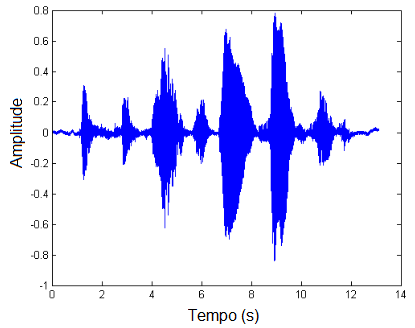
\includegraphics[width=0.6\textwidth]{img/exsinalsom.PNG}
\caption{\label{fig:exsinalsom}Exemplo de visualização de sinal sonoro, medindo a amplitude ao longo do tempo}
\author{Fonte: UNESP, Princípios de Comunicações, 2013}
\end{figure}

% \begin{figure}[]
% \centering
% 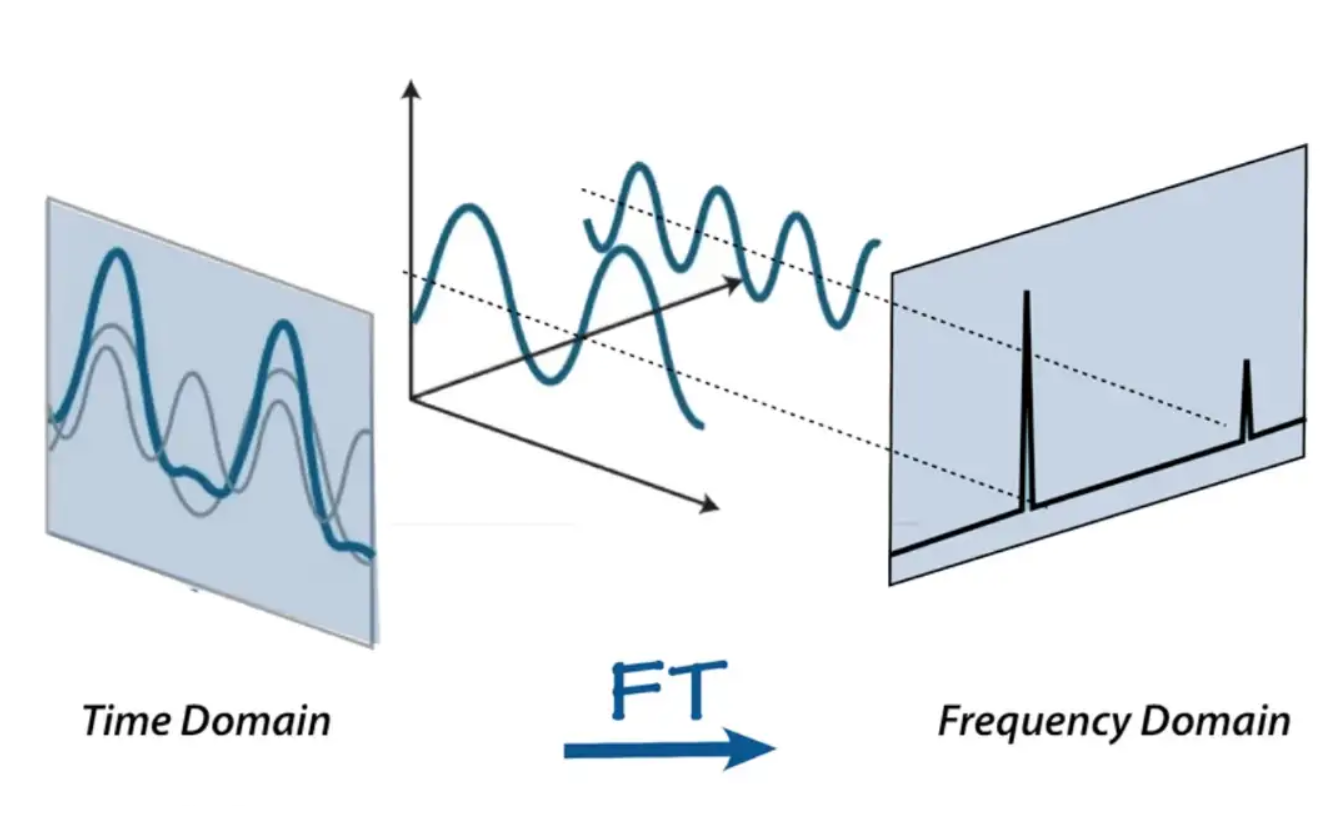
\includegraphics[width=0.6\textwidth]{img/ft.png}
% \caption{\label{fig:fouriertransform}Ilustração da Transformada de Fourier}
% \end{figure}

Com o resultado da \acrshort{TRF} de uma amostra, podemos calcular o seu espectrograma (\textit{spectrogram}): Uma representação da densidade das frequências ao longo do tempo. Entretanto, como humanos não compreendem todo o espectro sonoro~\cite{62}, será aplicada uma normalização às frequências, e calcularemos o Espectrograma de Mel (\textit{Mel-Spectrogram}).

% \footnote{No ano 2000 a \acrshort{FFT} foi incluída pela IEEE numa lista dos dez algoritmos mais influentes para o desenvolvimento e prática da ciência no século 20. Fonte: \textit{Guest Editors Introduction to the top 10 algorithms}. Disponível em \url{https://ieeexplore.ieee.org/document/814652/}}

% Na Figura\footnote{Disponível em \url{https://medium.com/analytics-vidhya/understanding-the-mel-spectrogram-fca2afa2ce53}}
%  \ref{fig:specvsmelespectrograma}, podemos observar a normalização das frequências (eixo vertical).

% https://towardsdatascience.com/learning-from-audio-the-mel-scale-mel-spectrograms-and-mel-frequency-cepstral-coefficients-f5752b6324a8

A normalização em questão, é a normalização pela Escala de Mel (\textit{Mel Scale}). Uma escala construída para tornar tons equidistantes perceptivelmente equidistantes ao ouvido humano. A Escala de Mel é dada por:

\begin{equation}
    m(f) = 1127 * \log_e{(1 + \frac{f}{700})}
\end{equation}

O \textit{Mel-Spectrogram} tem sido amplamente utilizado em problemas de \acrshort{SER}, como~\cite{32.25, 32.30}, e em~\cite{32.31} e~\cite{32.32}, que também utilizam técnicas de \textit{Autoencoder}.

Outro atributo observado na literatura são os Coeficientes Cepstrais de Frequência Mel (\acrshort{MFCC}s). Um \acrshort{MFC} é uma representação de curto prazo do espectro de potência de um som, assim, \acrshort{MFC}s são os coeficientes que formam os \acrshort{MFCC}s coletivamente. Calcular os \acrshort{MFCC}s consiste em aplicar a Transformada Discreta do Cosseno ao \textit{Mel-Spectrogram}. Podemos compreender os \acrshort{MFCC}s como uma compressão~\cite{64} do \textit{Mel Spectrogram}. Também encontramos trabalhos que utilizam \acrshort{MFCC}s em~\cite{32.79} e~\cite{32.89}, cujas arquiteturas contém uma Rede Neural Convolucional e uma \acrshort{GAN}, respectivamente.

% Podemos observar um comparativo entre o resultado de um Mel-Spectrogram e \acrshort{MFCC}s para uma mesma amostra na Figura \ref{fig:melspecvsmfcc}.

% \begin{figure}[]
% \centering
% 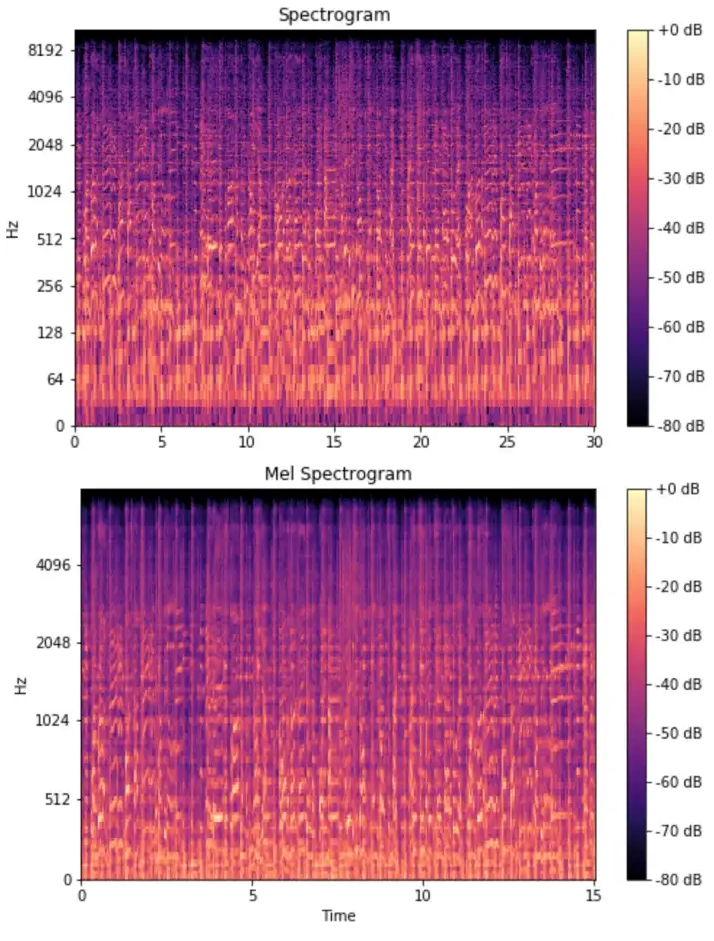
\includegraphics[width=0.6\textwidth]{img/espectrograma-vs-mel-espectrograma.png}
% \caption{\label{fig:specvsmelespectrograma}Exemplos de Espectrograma e Espectrograma de Mel}
% \end{figure}

% \begin{figure}[]
% \centering
% 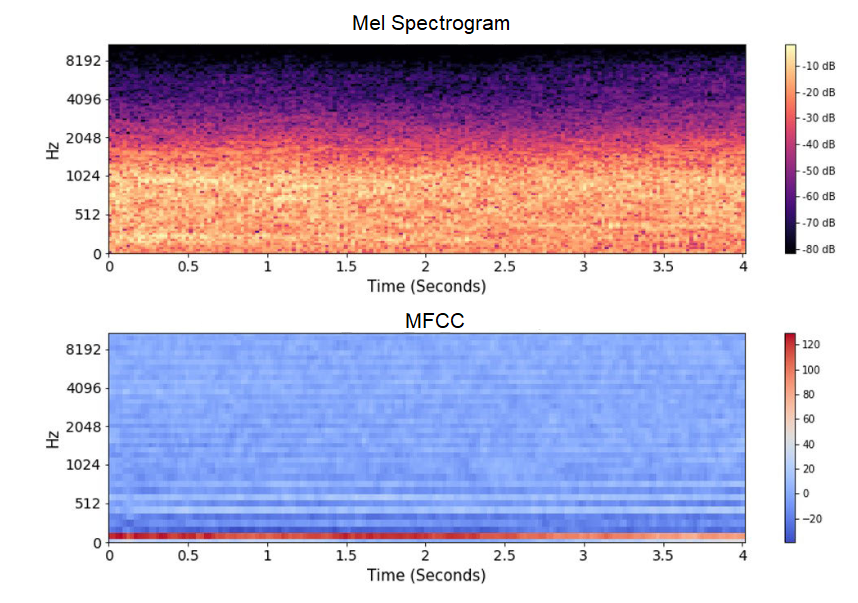
\includegraphics[width=0.6\textwidth]{img/melspec-vs-mfcc.PNG}
% \caption{\label{fig:melspecvsmfcc}Espectrograma de Mel e \acrshort{MFCC}s de uma mesma amostra sonora}
% \author{Fonte: Imagem adaptada de~\cite{64}}
% \end{figure}


Assim, sejam os dois \textit{datasets} VERBO e VIVAE, de modo que VERBO é constituído por pares \{amostra, classe\} e VIVAE por pares \{amostra, classe, intensidade\}, onde as classes são a emoção atribuída àquela amostra, e a intensidade é o rótulo da intensidade da classe daquela amostra. Vamos representar as amostras do VERBO por $X_{VERBO}$ e do VIVAE por $X_{VIVAE}$.

\begin{table}[]
\centering
\caption{Atributos dos datasets VERBO, VIVAE, ideal e da fusão de domínios}
\begin{tabular}{l|cccc|}
\cline{2-5}
 & \multicolumn{4}{c|}{Datasets} \\ \hline
\multicolumn{1}{|l|}{Atributos} & \multicolumn{1}{c|}{VERBO} & \multicolumn{1}{c|}{VIVAE} & \multicolumn{1}{c|}{Ideal} & Data Fusion(VERBO,VIVAE) \\ \hline
\multicolumn{1}{|l|}{Idioma} & \multicolumn{1}{c|}{X} & \multicolumn{1}{c|}{} & \multicolumn{1}{c|}{X} & X \\ \hline
\multicolumn{1}{|l|}{Emoções} & \multicolumn{1}{c|}{X} & \multicolumn{1}{c|}{X} & \multicolumn{1}{c|}{X} & X \\ \hline
\multicolumn{1}{|l|}{Intensidade} & \multicolumn{1}{c|}{} & \multicolumn{1}{c|}{X} & \multicolumn{1}{c|}{X} & X \\ \hline
\end{tabular}\label{table:datasetideal}
\end{table}

Em virtude da diferença da duração dos áudios entre VERBO e VIVAE, visando reduzir a quantidade de variáveis no problema, estes sinais foram empilhados horizontalmente uma quantidade inteira de vezes para tentar alcançar a maior duração (5s) entre as amostras, e o tempo restante foi preenchido com zeros.

Seja $Y_{VERBO}$ o conjunto das classes (emoções) $y_i \forall x_i \in X_{VERBO}$, analogamente para $Y_{VIVAE}$, vamos definir $Y = Y_{VERBO} \bigcap Y_{VIVAE}$. Vamos definir por por $Z$ o conjunto das intensidades. Uma vez que as intensidades estão apenas presentes em VIVAE, vamos utilizar suas quatro classes (baixa, moderada, forte, pico). Sabemos das Tabelas \ref{table:vivaeintensidade} e \ref{table:totalporclasse} que

\begin{itemize}
    \item $Y = \{alegria, medo, raiva, surpresa\}$
    \item $Z = \{baixa, moderada, forte, pico\}$
\end{itemize}

Vamos redefinir $X_{VERBO} = \{x_i \mid y_i \in Y\}$, analogamente para $X_{VIVAE}$, e vamos definir nosso domínio $X = X_{VERBO} \bigcap X_{VIVAE}$, assim

\begin{itemize}
    \item $\forall x_i \in X, \exists y_i \in Y$ tal que  $y_i$ é a classe de $x_i$
    \item $\forall x_j \in X_{VIVAE}, \exists z_j \in Z$ tal que  $z_j$ é a intensidade de $x_j$
\end{itemize}

Ao realizar tarefas de \acrshort{DL}, precisamos transformar os dados de entrada em um formato passível de ingestão pelos modelos. Os arquivos \textit{.wav} de $X$ serão lidos e iremos gerar seus respectivos \acrshort{MFC}s, convertendo o sinal de áudio ao longo do tempo para uma representação do sinal no domínio da frequência, que será utilizada pelos modelos. Então, teremos um mapa $M(x_i): MFC_i$.


% ==========================================================================================
\section{Extração de características}

De posse do mapa $M(x_i)$, podemos prosseguir para a etapa de extração de características. Uma vez que $X$ é formado por dados de \textit{datasets} diferentes, buscamos uma forma de extrair características relevantes com boa capacidade de generalização ao ser aplicada em ambos $X_{VERBO}$ e $X_{VIVAE}$.

% ------------------------------------------------------------------------------------------
\subsection{Codificador Automático}

Um Codificador Automático (\acrshort{AE}) é uma rede neural criada para tentar reproduzir o seu \textit{input} no seu \textit{output}. Podemos descrever um \acrshort{AE} como um conjunto de funções $f, f'$ de modo que, dado um input $x$, queremos $f'(f(x)) = x' \approx x$, onde $f$ realiza a codificação (\textit{encoding}) de $x$ e $f'$ realiza a decodificação (\textit{decoding}) do resultado $f(x)$. Assim, um \acrshort{AE} é uma rede neural composta por um \textit{encoder} e um \textit{decoder} que tenta reproduzir uma função de identidade.

% (Figura\footnote{Imagem adaptada, gerada em \url{http://alexlenail.me/NN-SVG/LeNet.html}} \ref{fig:exarqae})

O resultado da etapa de \textit{encoding} costuma ter uma dimensionalidade menor do que a do dado de entrada. O espaço composto por dados codificados (\textit{encoded}) é chamado de Espaço Latente (\textit{Latent Space}), um espaço composto por representações significativas dos dados, contendo informações sobre cada amostra que possivelmente não estariam visíveis nas representações de alta dimensionalidade~\cite{60}.

Entretanto, \acrshort{AE}s não podem simplesmente aprender a generalizar $f'(f(x)) = x$ para todo tipo de dado, ao invés disso, são impostas restrições para que consigam esse tipo de generalização apenas para os dados relevantes a sua tarefa. Forçando o modelo a priorizar características que devem ser aprendidas, por vezes, ele aprende propriedades úteis sobre os dados.

Tradicionalmente, \textit{Autoencoder}s foram utilizados para reduzir a dimensionalidade de dados (\textit{dimensionality reduction}) ou para aprender características (\textit{feature learning}) sobre os dados. Atualmente, \acrshort{AE}s são bastante utilizados como peça fundamental em Redes Generativas Adversariais (\acrshort{GAN}) e \textit{Autoencoder}s Variacionais (\acrshort{VAE}).

% \footnote{Introduzido em 2013 por Diederik P Kingma e Max Welling. Disponível em \url{https://arxiv.org/abs/1312.6114}}

% \footnote{Introduzido em 2014 por Ian J. Goodfellow \textit{et al.}. Disponível em \url{https://arxiv.org/abs/1406.2661}}

% \begin{figure}[!h]
% \centering
% 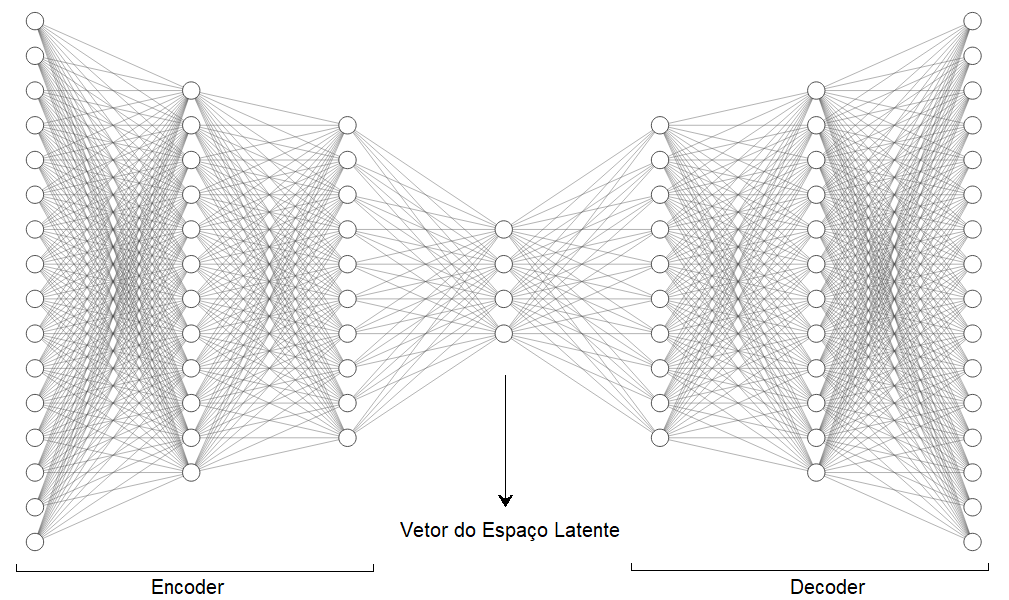
\includegraphics[width=0.6\textwidth]{img/ex-ae.PNG}
% \caption{\label{fig:exarqae}Exemplo de arquitetura \acrshort{AE}}
% \end{figure}

% Apesar da representação visual, os \textit{MFCC}s formam um vetor de alta dimensionalidade.

Redes neurais constituem uma boa ferramenta para tarefas de \acrshort{SER}. \acrshort{AE}s, podem criar uma representação de qualidade com dimensionalidade reduzida em seu espaço latente, enquanto \acrshort{DNN}s encontram espaço na literatura como bons discriminadores ou classificadores.

Vamos construir um \acrshort{AE}, ilustrado na Figura \ref{fig:composicaoae}, que tenta reproduzir uma função identidade. Por definição, um \acrlong{AE} é composto por uma função \textit{encoder} ($f_e$) e uma função $decoder$ ($f_d$), de modo que $AE: M \rightarrow M'$ faça

\begin{equation}
    AE(x) = f_d(f_e(x)) = x' \approx x
\end{equation}

\begin{figure}[]
    \centering
    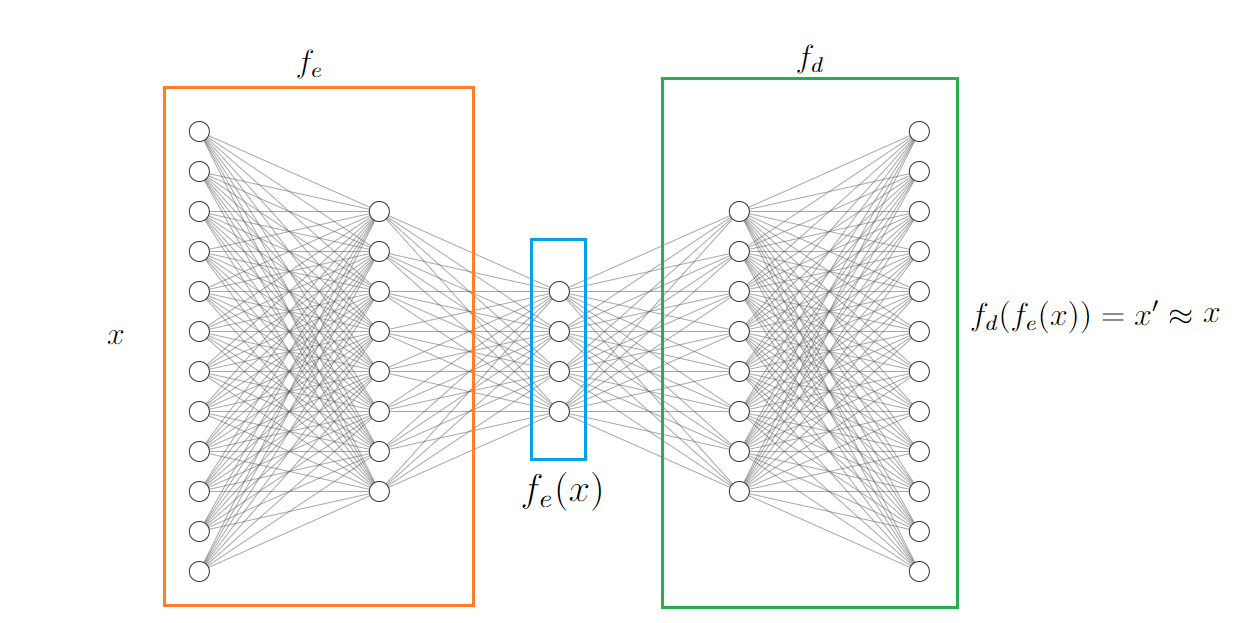
\includegraphics[width=0.8\textwidth]{img/p-autoencoder.png}
    \caption{\label{fig:composicaoae}Composição do \acrshort{AE}}
\end{figure}

Para o treinamento do modelo $AE$ com os dados de $X$, este será dividido em um conjunto de treino e outro de teste, contendo 75\% e 25\% dos registros de $X$, respetivamente. Em seu espaço latente teremos uma representação do dado de entrada com a dimensionalidade reduzida, preservando suas características de maneira suficiente para que possa ser reconstruído ($x'$) ao aplicar a função de \textit{decoding}.

A estrutura dos Autoencoders é análoga para ambos os experimentos. A Figura \ref{fig:ae64} representa a arquitetura do modelo para 64 \acrshort{MFCC}s enquanto a \ref{fig:ae128} representa a arquitetura do modelo para 128 \acrshort{MFCC}s. Ambos seguem uma estrutura composta por três camadas, a serem detalhadas abaixo: Entrada, \textit{encoder} e \textit{decoder}.

O treinamento foi realizado utilizando o Erro Quadratico Médio (\acrshort{MSE}) como função de Perda (\textit{Loss}) e \acrshort{ADAM} como função de otimização. Para efeitos de legibilidade, vamos definir $dim_{MFCCs}$ como a quantidade de \acrshort{MFCC}s utilizado em cada experimento.

\begin{enumerate}
    \item Entrada: Responsável por receber os dados com dimensão igual $(1, dim_{MFCCs})$.
    \item \textit{Encoder}: Responsável por realizar a redução de dimensionalidade do dado oriundo da camada de entrada. Na camada de \textit{encoder}, o dado entra com dimensão $(1, dim_{MFCCs})$ e é comprimido para uma dimensionalidade $(1, dim_{MFCCs}/2)$. Assumimos que buscamos preservar apenas os atributos com maior relevância, então utilizamos uma função de ativação do tipo Unidade Linear Retificada (\acrshort{ReLU}).
    \item \textit{Decoder}: Responsável por receber os dados com dimensão reduzida e expândi-los para a dimensão de entrada $(1, dim_{MFCCs})$, tentando reproduzir os valores originais. Para isso, esta camada utilizou uma função de ativação do tipo Linear, que reproduzirá valores contítnuos oriundos das operações matriciais desta camada, não limitados ao intervalo $(0, max(0, x)$ como é o caso da \acrshort{ReLU}.
\end{enumerate}

% ---- Arquiteturas AEs ---- %
\begin{figure}[h]
    \centering
    \begin{minipage}[b]{0.4\linewidth}
        \centering
        \includegraphics[width=\linewidth]{img/ae64.png}
        \caption{\label{fig:ae64}Arquitetura do Autoencoder para 64 \acrshort{MFCC}s}
    \end{minipage}
    % \hfill
    \begin{minipage}[b]{0.4\linewidth}
        \centering
        \includegraphics[width=\linewidth]{img/ae128.png}
        \caption{\label{fig:ae128}Arquitetura do Autoencoder para 128 \acrshort{MFCC}s}
    \end{minipage}
\end{figure}


% ------------------------------------------------------------------------------------------
\subsection{Validação}

Antes de seguir para a etapa de classificação (B), precisamos verificar a qualidade do modelo produzido, já que este irá prover os dados para o próximo modelo. Apesar de ser um modelo não supervisionado, podemos pensar em formas de aferir seu desempenho. Uma vez que o modelo \acrshort{AE} tenta reproduzir a função identidade, podemos calcular a diferença entre os atributos de entrada e os atributos de saída. Para isso, podemos utilizar o Erro Quadrático Médio (\acrshort{MSE}):

\begin{equation}
    MSE = \frac{1}{n} * \sum^n_{i=1} (x_i - x'_i)^2
\end{equation}

É desejado que o \acrshort{MSE} para os atributos de $\{x, x'\}$ seja o mais próximo de zero, indicando que o modelo consegue reconstruir o \textit{input} com grande precisão.


% ==========================================================================================
\section{Classificação da Intensidade}

                    % !!! por algum motivo esse parágravo causa erro de compilação !!! %
% Através do modelo de Russel sabemos que que é possível dispor as emoções em função da valência (prazer ou desprazer) e da ativação (vigor ou quietude) \cite{27}. Plutchik decompõe as emoções básicas de acordo com a intensidade, chegando a emoções compostas, formadas a partir de duas emoções com intensidades menores.

% Ao longo do Capítulo 3, observamos trabalhos relacionados, desafios pertinentes à pesquisa e o estado da arte na área de estudo deste trabalho, que se diferencia dos pares por, além de ser um dos poucos trabalhos a lidar com o idioma português, também aborda a questão da intensidade da emoção.

% Sabemos da relevância que \textit{features} espectrais carregam sobre a vocalização e vimos formas para avaliar o desempenho dos modelos.

Redes neurais são capazes de aprender relações complexas entre as características dos dados, o que pode ser especialmente benéfico para a tarefa de classificação. Ao contrário de métodos mais tradicionais, as redes neurais não estão limitadas por suposições lineares ou por características específicas pré-definidas, permitindo uma modelagem mais flexível e adaptativa dos dados.

Com o \textit{Autoencoder} treinado, vamos aplicá-lo a todos os registros de $X_{VIVAE}$ e separar o resultado em dois conjuntos para treinamento ($X_{VIVAE_{treino}}$) e testes ($X_{VIVAE_{teste}}$), contendo 75\% e 25\% desses dados, respectivamente. Estes serão os dados utilizados pelo nosso modelo supervisionado.

% Para a etapa de classificação da intensidade (C), construímos e treinamos uma rede neural $j$, que recebe como \textit{input} o \textit{encoding} da média dos \textit{MFC}s dos $x_i \in X_{VIVAE_{treino}}$.

Este modelo (Figura \ref{fig:jsupervisionado}) foi construído para classificar a intensidade da emoção de forma direta. Uma vez que os $x_i \in X_{VIVAE_{treino}}$ têm correspondentes em $Z$, contradomínio das intensidades, então, $j: M \rightarrow Z$, é tal que $j(f_e(m)) = z$

\begin{figure}[h]
    \centering
    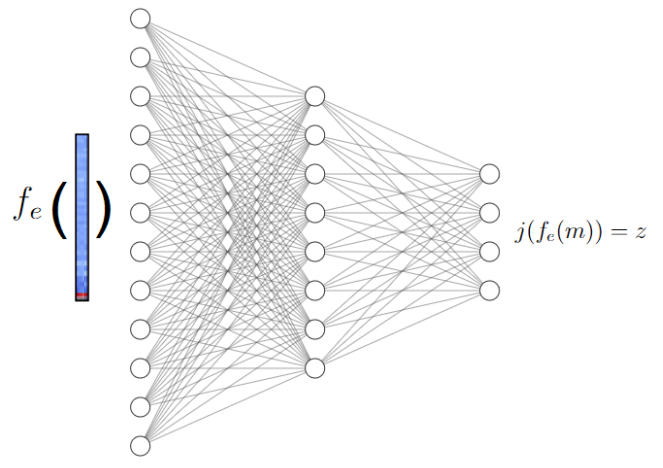
\includegraphics[width=0.75\textwidth]{img/p-supervisionado.png}
    \caption{\label{fig:jsupervisionado}Modelo supervisionado $j$}
\end{figure}


A estrutura dos Classificadores é análoga para ambos os experimentos. A Figura \ref{fig:clf64} representa a arquitetura do modelo para 64 \acrshort{MFCC}s enquanto a \ref{fig:clf128} representa a arquitetura do modelo para 128 \acrshort{MFCC}s. Ambos seguem uma estrutura composta por cinco camadas, a serem detalhadas abaixo: Entrada, três camadas densas intermediárias e uma camada densa de saída.

O treinamento foi realizado utilizando \textit{Categorical Cross Entropy} como função de \textit{Loss} e \acrshort{ADAM} como função de otimização. Uma vez que o \acrshort{AE} realiza a função de reduzir a dimensionalidade dos dados que serão utilizados como \textit{input} para os classificadores, para efeitos de legibilidade vamos definir $dim_{encode}$ como a dimensão do dado comprimido obtido nos \textit{Autoencoders} da etapa anterior, sendo estas 32 e 64, respectivamente.

\begin{enumerate}
    \item Entrada: Responsável por receber os dados com dimensão igual $(1, dim_{encode})$.
    \item Densas intermediárias: As camadas posteriores (\textit{dense}, \textit{dense\_1} e \textit{dense\_2}) são camadas totalmente conectadas que utilizam a função de ativação \acrshort{ReLU} e cujo resultado é um vetor com dimensão $(1, 8)$.
    \item Densa de saída: A camada \textit{dense\_3} é responsável por efetuar a ativação final da rede neural e entrega um vetor com dimensão $(1, 4)$. Utiliza uma função de ativação \textit{Softmax}, cujo resultado será interpretado para classificar a intensidade da emoção em uma de quatro categorias: Fraca, moderada, forte ou pico de intensidade.
\end{enumerate}

% ---- Arquiteturas CLFs ---- %
\begin{figure}[]
    \centering
    \begin{minipage}[b]{0.45\linewidth}
        \centering
        \includegraphics[width=\linewidth]{img/clf64.png}
        \caption{\label{fig:clf64}Arquitetura do classificador do experimento com 64 \acrshort{MFCC}s}
    \end{minipage}
    % \hfill
    \begin{minipage}[b]{0.45\linewidth}
    \centering
        \includegraphics[width=\linewidth]{img/clf128.png}
        \caption{\label{fig:clf128}Arquitetura do classificador do experimento com 128 \textit{MFCC}s}
    \end{minipage}
\end{figure}


% ------------------------------------------------------------------------------------------
\subsection{Validação}

Por ser tratar de um modelo supervisionado, podemos aplicar as métricas descritas no Capítulo 2, utilizando $X_{VIVAE_{teste}}$ para observar seus resultados. Neste trabalho, perceberemos um erro de  falso negativo de maneira equivalente a um erro de falso positivo. Portanto, não buscamos otimizar as métricas como \textit{Precision} ou \textit{Recall}. Assim, utilizaremos utilizaremos \textit{F1-Score} como parâmetro de desempenho para o modelo supervisionado.
